\documentclass[a4paper,10pt]{article}
%\usepackage[utf8x]{inputenc}
\usepackage{listings}
\usepackage{color}
\usepackage{graphicx}

%opening
\title{OpenDA course and exercises}
\author{Nils van Velzen, Martin Verlaan, Stef Hummel}

\begin{document}
\lstset{ %
 basicstyle=\ttfamily,            % the size of the fonts that are used for the code
 breakatwhitespace=false,         % sets if automatic breaks should only happen at whitespace
 breaklines=true,                 % sets automatic line breaking
 captionpos=b,                    % sets the caption-position to bottom
 columns=flexible, 		    				% Prevent additional spaces to be entered by the listing, when keepspaces = true --> enable copy - paste
 escapeinside={\%*}{*)},          % if you want to add LaTeX within your code
 extendedchars=true,              % lets you use non-ASCII characters; for 8-bits encodings only, does not work with UTF-8
 frame=single,	                  % adds a frame around the code
 keepspaces=true,                 % keeps spaces in text, useful for keeping indentation of code (possibly needs columns=flexible)
 numbers=none,                    % where to put the line-numbers; possible values are (none, left, right)
 numbersep=5pt,                   % how far the line-numbers are from the code
 numberstyle=\tiny\color{mygray}, % the style that is used for the line-numbers
 showspaces=false,                % show spaces everywhere adding particular underscores; it overrides 'showstringspaces'
 showstringspaces=false,          % underline spaces within strings only
 showtabs=false,                  % show tabs within strings adding particular underscores
 tabsize=2,	                      % sets default tabsize to 2 spaces
}

\maketitle

%\begin{abstract}

%\end{abstract}

\section*{Installation of OpenDA}
Before you can start with the exercises you must first install OpenDA. For the
latest instructions, you are referred to \verb|$OPENDA/doc/OpenDA_domunentation.pdf|, 
section "Installation" or the same document on our website \verb|www.openda.org|.

For postprocessing with python we assume that the numpy and pyplot modules are loaded. If not, then you
can do this with the commands:
      \begin{lstlisting}[language=Python,frame=single,caption={Python initialize}]
      import numpy as np
      import matplotlib.pyplot as plt
      \end{lstlisting}
Please type (or copy-paste) onto the python prompt.

\section{Exercise 1 part1: Getting started}

A pendulum is a rigid body that can swing under the influence of gravity. It is attached at the top so it can roatate freely in a two-dimensional plane ($x,y$).
We will assume a thin rectangular shape with the mass equally distributed. A double pendulum is a pendulum connected to the end of another pendulum. Contrary to the 
regular movement of a pendulum, the motion of a double-pendulum is very irregular when sufficient energy is put into the system. 

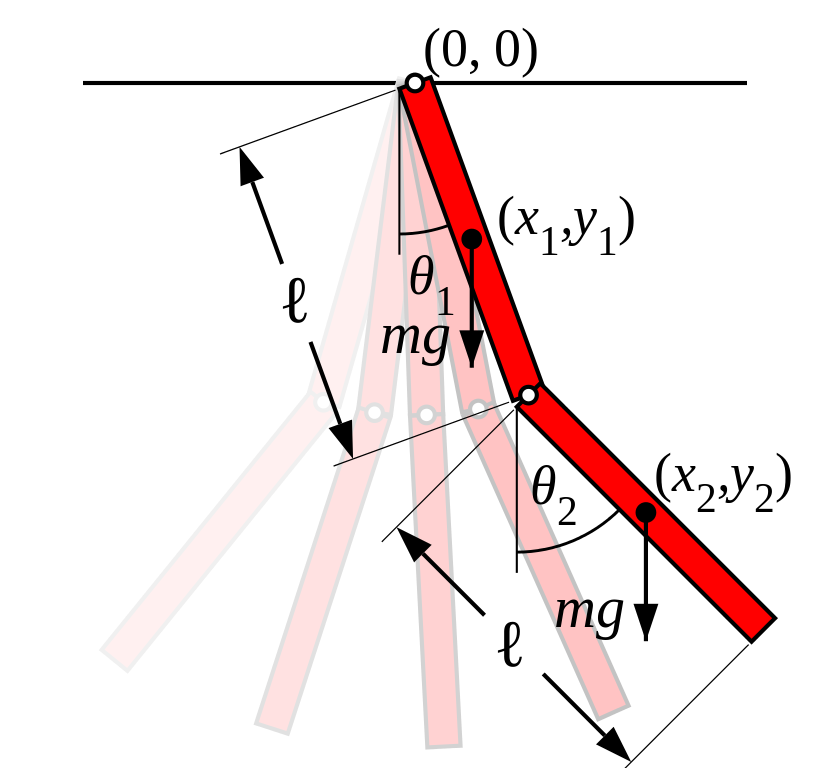
\includegraphics[height=4cm]{Double-compound-pendulum.png}

The dynamics of a double-pendulum can be descibed with the following equations 
( This example was copied from https://en.wikipedia.org/wiki/Double\_pendulum )

variables $\theta_1, \theta_2, p_{\theta_1}, p_{\theta_2}$:
\begin{eqnarray}
   \frac{d \theta_1}{dt}= \frac{6}{m l^2} \frac{2 p_{\theta_1} - 3cos(\theta_1-\theta_2) p_{\theta_2}}
   {16-9 cos^2(\theta_1-\theta_2)}\\
   \frac{d \theta_2}{dt}= \frac{6}{m l^2} \frac{8 p_{\theta_2} - 3cos(\theta_1-\theta_2) p_{\theta_1}}
   {16-9 cos^2(\theta_1-\theta_2)}\\
   \frac{dp_{\theta_1}}{dt} = -\frac{1}{2} ml^2 \left( \frac{d \theta_1}{dt} \frac{d \theta_2}{dt} sin(\theta_1-\theta_2) + 3\frac{g}{l} sin(\theta_1) \right)  \\
   \frac{dp_{\theta_1}}{dt} = -\frac{1}{2} ml^2 \left( -\frac{d \theta_1}{dt} \frac{d \theta_2}{dt} sin(\theta_1-\theta_2) + \frac{g}{l} sin(\theta_2) \right) 
\end{eqnarray}
where the $x,y$-position of the middle of the two segments can be computed as:
\begin{eqnarray}
   x_1 = \frac{l}{2} sin(\theta_1) \\
   y_1 = \frac{-l}{2} cos(\theta_1) \\
   x_2 = l ( sin(\theta_1) + \frac{1}{2} sin(\theta_2) ) \\
   y_2 = -l ( cos(\theta_1) + \frac{1}{2} cos(\theta_2) )
\end{eqnarray}

This model, although simple, is very nonlinear and has a chaotic nature.  Its
solution is very sensitive to the parameters and the initial conditions: a
small difference in those values can lead to a very different solution.

The purpose of this exercise is to get you started with OpenDA. You will learn
to run a model in OpenDA, make modifications to the input files and plot the
results.

\begin{itemize}
\item The input for this exercise is located in directory \texttt{ exercise\_pendulum\_part1}.
      For Linux and Mac OS X, go to this directory and start \texttt{ oda\_run.sh}, the
      main application of OpenDA. For Windows, start the main application with 
      \texttt{ oda\_run\_gui.bat} from the \texttt{ \$OPENDA/bin} directory. The main 
      application allows you to view and edit the OpenDA configuration files, run your
      simulations and visualize the results.
\item Try to run a simulation with the double pendulum model. You can use the
      configuration file \texttt{ simulation\_unperturbed.oda}. 
      
      For postprocessing in Matlab the results are written to \\ \texttt{ simulation\_unperturbed\_results.m}.
      Next start Matlab and load the results. We have added a routine \texttt{ plot\_movie} to create an intuitive
      representation of the data. Please type (or copy-paste):
      \begin{lstlisting}[language=Matlab,frame=single,caption={Matlab}]
      [t,unperturbed,tobs,obs]= ...
      load_results('simulation_unperturbed_results');
      plot_movie(t,unperturbed)
      \end{lstlisting}
      
      For postprocessing in Python the results are written to \\ \texttt{ simulation\_unperturbed\_results.py}.
      These results can be loaded with:
      \begin{lstlisting}[language=Python,frame=single,caption={Python initialize}]
      import simulation_unperturbed_results as unperturbed
      # use reload(unperturbed) if unperturbed was loaded before
      \end{lstlisting}
      We have added a routine \texttt{ plot\_movie} to create an intuitive
      representation of the data. 
      \begin{lstlisting}[language=Python,frame=single,caption={Python}]
      import pendulum as p #needed only once
      p.plot_movie(unperturbed.model_time,unperturbed.x)
      \end{lstlisting}
      
      To create a time-series plot in Matlab type:
      \begin{lstlisting}[language=Matlab,frame=single,caption={Matlab}]
       subplot(2,1,1);
       plot(t,unperturbed(1,:),'b-');
       ylabel('\theta_1');
       subplot(2,1,2);
       plot(t,unperturbed(2,:),'b-');
       ylabel('\theta_2');
       xlabel('time');
      \end{lstlisting}
      
      To create a time-series plot in Python type:
      \begin{lstlisting}[language=Python,frame=single,caption={Python}]
      plt.subplot(2,1,1)
      plt.plot(unperturbed.model_time,unperturbed.x[:,0],'b') #python counts starting at 0
      plt.ylabel(r'$\theta_1$') # use raw string and latex for label
      plt.subplot(2,1,2)
      plt.plot(unperturbed.model_time,unperturbed.x[:,1],'b')
      plt.ylabel(r'$\theta_2$')
      plt.show() #only needed if interactive plotting is off. Set with plt.ioff(), plt.ion()
      \end{lstlisting}
%


\item Then you can start an alternative simulation with the double-pendulum model that
       starts with a slightly different initial condition using the
       configuration file \texttt{ simulation\_perturbed.oda}. The different initial conditions
       can be found in \texttt{model\/DoublePendulumStochModel.xml} and \\
       \texttt{model\/DoublePendulumStochModel\_perturbed.xml}

\item  Visualize the unperturbed and perturbed results in a single plot. Make
       a movie and a time-series plot of $\theta_1$ and $\theta_2$ variables. Do you see
       the solutions diverging like the theory predicts?
       
      \begin{lstlisting}[language=Matlab,frame=single,caption={Matlab}]
       [tu,unperturbed,tobs1,obs1]=load_results('simulation_unperturbed_results');
       [tp,perturbed,tobs2,obs2]=load_results('simulation_perturbed_results');
       figure(1);clf;subplot(2,1,1);
       plot(tu,unperturbed(1,:),'b');
       hold on;
       plot(tp,perturbed(1,:),'g');
       hold off;
       legend('unperturbed','perturbed')
       subplot(2,1,2);
       plot(tu,unperturbed(2,:),'b');
       hold on;
       plot(tp,perturbed(2,:),'g');
       hold off;
      \end{lstlisting}
      
      To create a movie with both results in python type:
      \begin{lstlisting}[language=Python,frame=single,caption={Python initialize}]
      import simulation_unperturbed_results as unperturbed
      import simulation_perturbed_results as perturbed
      p.plot_movie(unperturbed.model_time,unperturbed.x,perturbed.x)
      \end{lstlisting}

      To create a time-series plot with both results in Python type:
      \begin{lstlisting}[language=Python,frame=single,caption={Python}]
      plt.subplot(2,1,1)
      plt.plot(unperturbed.model_time,unperturbed.x[:,0],'b') #python counts starting at 0
      plt.plot(perturbed.model_time,perturbed.x[:,0],'g') #python counts starting at 0
      plt.ylabel(r'$\theta_1$') # use raw string and latex for label
      plt.subplot(2,1,2)
      plt.plot(unperturbed.model_time,unperturbed.x[:,1],'b')
      plt.plot(perturbed.model_time,perturbed.x[:,1],'g')
      plt.ylabel(r'$\theta_2$')
      plt.show() 
      \end{lstlisting}
      
\item Next we want to create an ensemble of model runs all with slightly different initial conditions. 
      You can do this in a number of steps:
      \begin{itemize}
      \item First create the input file \texttt{ simulation\_ensemble.oda} based on\\
            \texttt{ simulation\_unperturbed.oda}. Change the algorithm and the
            configuration of the algorithm.\\
            hint: the algorithm is called \\
            org.openda.algorithms.kalmanFilter.SequentialEnsembleSimulation.
      \item Create a configuration file for the Ensemble algorithm (e.g. named
            \texttt{ algorithm/SequentialEnsembleSimulation.xml}) with the following content:
      \begin{lstlisting}[language=XML,frame=single,caption={XML-input for sequentialAlgorithm}]
      <?xml version="1.0" encoding="UTF-8"?>
      <sequentialAlgorithm>
         <analysisTimes type="fromObservationTimes" ></analysisTimes>
         <ensembleSize>5</ensembleSize>
         <ensembleModel stochParameter="false"
                        stochForcing="false"
                        stochInit="true" />
      </sequentialAlgorithm>
      \end{lstlisting}
      Hint: do not forget to reference \texttt{ algorithm/SequentialEnsembleSimulation.xml} in \\ \texttt{ simulation\_ensemble.oda}
      and do not forget to give a diferent name to the output files.
      \item Run the new configuration with OpenDA.

      \item make a plot of the first and second variable of the five ensemble
      members in a single time-series plot
      \begin{lstlisting}[language=Matlab,frame=single,caption={Matlab}]
      [t,ens]=load_ensemble('simulation_ensemble_results');
      ens_th1=reshape(ens(1,:,:),size(ens,2),size(ens,3));
      ens_th2=reshape(ens(2,:,:),size(ens,2),size(ens,3));
      clf; subplot(2,1,1);
      plot(t(2:end),ens_th1);
      ylabel('\theta_1');
      subplot(2,1,2);
      plot(t(2:end),ens_th2);
      ylabel('\theta_2');
      xlabel('time');
      \end{lstlisting}
      
      \begin{lstlisting}[language=Python,frame=single,caption={Python}]
      import ensemble
      import simulation_ensemble_results as res
      (t,ens)=ensemble.reshape_ensemble(res)
      ens1=ens[:,0,:] #note we start counting at 0
      ens2=ens[:,1,:]
      plt.subplot(2,1,1)
      plt.plot(t[1:],ens1,'b')
      plt.ylabel(r'$\theta_1$')
      plt.subplot(2,1,2)
      plt.plot(t[1:],ens2,'b')
      plt.ylabel(r'$\theta_2$')
      plt.show()
      \end{lstlisting}
      
      \item Observations of $\theta_1$ and $\theta_2$ are available as well. Make a plot of
      the observations together with the simulation results.
      \begin{lstlisting}[language=Matlab,frame=single,caption={Matlab}]
	[t,unperturbed,tobs,obs]= ...
	load_results('simulation_unperturbed_results');
       subplot(2,1,1);
       plot(t,unperturbed(1,:),'b-');
       hold on
       plot(tobs,obs(1,:),'k+');
       hold off
       ylabel('\theta_1');
       subplot(2,1,2);
       plot(t,unperturbed(2,:),'b-');
       hold on
       plot(tobs,obs(2,:),'k+');
       hold off
       ylabel('\theta_2');
       xlabel('time');
      \end{lstlisting}
      \begin{lstlisting}[language=Python,frame=single,caption={Python}]
      import simulation_unperturbed_results as unperturbed
      plt.subplot(2,1,1)
      plt.plot(unperturbed.model_time,unperturbed.x[:,0],'b') #python counts starting at 0
      plt.plot(unperturbed.analysis_time,unperturbed.obs[:,0],'k+') #python counts starting at 0
      plt.ylabel(r'$\theta_1$') # use raw string and latex for label
      plt.subplot(2,1,2)
      plt.plot(unperturbed.model_time,unperturbed.x[:,1],'b')
      plt.plot(unperturbed.analysis_time,unperturbed.obs[:,1],'k+')
      plt.ylabel(r'$\theta_2$')
      plt.show()
      \end{lstlisting}
      
      We can see that although our simulation starts on the right track, it quickly diverges from the observations.
      The aim of the Ensemble Kalman filter or data-assimilation in general, is to keep the model on track. 
      \end{itemize}

\end{itemize}


\section{Exercise 1 part 2: Some basic properties of the EnKF}

In this exercise you will learn how to set up and run the EnKF method in OpenDA.

\begin{itemize}
  \item Prepare the input files for a run with the EnKF method. Use the input
        files from exercise 1 as template. Hint: the Ensemble Kalman filter
        is called org.openda.algorithms.kalmanFilter.EnKF. The algorithm
        configuration file has the following content
      \begin{lstlisting}[language=XML,frame=single,caption={XML-input for EnKF algorithm}]
      <?xml version="1.0" encoding="UTF-8"?>
      <EnkfConfig>
         <ensembleSize>10</ensembleSize>
         <ensembleModel stochParameter="false"
                        stochForcing="false"
                        stochInit="true" />
      </EnkfConfig>
      \end{lstlisting}
      Note that we are considering only uncertainty of the initial conditions here. In general, also uncertainty of the 
      parameters or the model forcing, such as boundary conditions can be considered.

  \item Plot the ensemble mean of the first model variable and the observations.
        With some luck the solution should track the observations. \\
        For comparison we have also added the configurations for the 'truth' and a oda\_run
        without data-assimilation called 'initial'.
        
        \begin{lstlisting}[language=Matlab,frame=single,caption={Matlab}]
        [tt,truth,tobs1,obs1]=load_results('simulation_truth_results');
        [ti,initial,tobs2,obs2]=load_results('simulation_initial_results');
        [te,enkf,tobs2,obs2]=load_results('simulation_enkf_results');
        figure(1);clf;subplot(2,1,1);
        plot(tt,truth(1,:),'k');
        hold on;
        plot(ti,initial(1,:),'g');
        plot(te,enkf(1,1:2:end),'b');
        hold off;
        legend('truth','initial','enkf')
        subplot(2,1,2);
        plot(tt,truth(2,:),'k');
        hold on;
        plot(ti,initial(2,:),'g');
        plot(te,enkf(2,1:2:end),'b');
        hold off;
        \end{lstlisting}

        \begin{lstlisting}[language=Python,frame=single,caption={Python initialize}]
        import simulation_truth_results as truth
        import simulation_initial_results as initial
        import simulation_enkf_results as enkf
        plt.subplot(2,1,1)
        plt.plot(initial.model_time,initial.x[:,0],'g')
        plt.plot(truth.model_time,truth.x[:,0],'k')
        plt.plot(enkf.analysis_time,enkf.x_f_central[::2,0],'b');
        plt.legend(('initial','truth','EnKF'))
        plt.ylabel(r'$\theta_1$')
        plt.subplot(2,1,2)
        plt.plot(initial.model_time,initial.x[:,1],'g')
        plt.plot(truth.model_time,truth.x[:,1],'k')
        plt.plot(enkf.analysis_time,enkf.x_f_central[::2,1],'b');
        plt.ylabel(r'$\theta_2$')
        plt.xlabel(r'$t$')
        plt.show() 
        \end{lstlisting}

 \item The Ensemble Kalman filter is uses a random number generator. In OpenDA we can control 
       the initial value of the generator by adding a line like:
       \verb|<initialSeed type="specify" seedValue="21" />| near the end of the main configuration file.
       Do you get the same results if you rerun with the same value of the initial seed? And what if 
       you use a different value?
        
 \item Look at the observation input file of the StochObserver. The
       StochObserver does not only describe the observations but the accuracy
       as well. Can you make a new observation input file with similar
       observed values but with a 10 times larger standard deviation for the
       observation error.
       Tip: you can edit the file in OpenOffice or MS Excel or use the find
       and replace function of an advanced text editor.
       Repeat the run with EnKF but now for the new observations and plot
       the first variable of the ensemble means and the observations. What do
       you see and what is the reason for this behavior of the algorithm?
 %oda_run EnKf10.oda
 %plot1.m
 \item The number of ensemble members controls the accuracy of the ensemble
       approximation. What happens if you decrease it to 10 or 6? 
       
\end{itemize}

%extra: Belang van initial seed (een enkele run is ook maar een enkele realisatie) en gebruik van "ensembles van ensembles"
%laat ze ook spelen met initiele seed van de randomgenerator (kan dat in OpenDA??) Zodat ze dan zien dat voor grote ensembles minder impact (zou moeten) hebben dan voor kleine aantallen ensembles.



\section{Exercise 2: Localization}
In this exercise you will learn about localization techniques and how to use them in OpenDA. This exercise is inspired on the example model and experiments from "Impacts of localisation in the EnKF and EnOI: experiments with a small model", Peter R. Oke, Pavel Sakov and Stuart P. Corney, Ocean Dynamics (2007) 57: 32-45.

The model we use is a simple circular advection model 
\begin{equation}
\frac{\partial a}{\partial t}+u\frac{\partial a}{\partial x}=0
\end{equation}
where u=1 is the speed of advection, a is a model variable , t is time and x is a space ranging from 1 to 1000 with grid spacings of 1. The computational domain is periodic in x.

In this model there are two related variables a and b where b is initialised with a balance relationship:
\begin{equation}\label{eg:b_relation}
b= 0.5 + 10 \frac{da}{dx}
\end{equation}
and propagated with an advection model similar to the one for a, i.e.:
\begin{equation}
\frac{\partial b}{\partial t}+u\frac{\partial b}{\partial x}=0
\end{equation}
Since $a$ and $b$ are propagated with the same flow, the balance relationship will remain valid also for $t>0$.
The relation ship between a and b is motivated by the geostrophic balance relationship between pressure (a) and velocity (b) in oceanographic and atmospheric applications. 

In this experiment we will only observe and assimilate $a$ and investigate how both $a$ as $b$ are updated. 
The ensemble is carefully constructed in order to have the right statistics. The initial ensembles are generated off line and they will be read when the model is initialised in OpenDA. 

\begin{itemize}
\item Investigate the sript {\tt generate\_ensemble.py} and figure out how the ensembles are generated.
\item Run python script {\tt generate\_ensemble.py} to generate ensembles, observations and true state for a 25, 50 and 100 ensemble experiment.  
\item Run the experiment for 50 ensemble members ({\tt enkf\_50.oda}).
\item The variables $a$, $b$ can be compared to the true state using the python script {\tt plot\_results.py}.
\item Run the experiment for 25 ensembles, copy the script {\tt plot\_results.py} to e.g. {\tt plot\_results\_25.py} and adjust it in order to read the results from {\tt enkf25\_results.py}.
(change 2nd line of the {\tt plot\_results.py} script. You will see that the 25 ensemble run is not able to improve the model.
\item Create input to run a 100 ensemble experiment. Note: do not forget to change the name of the output file (section {\tt resultWriter}) 
to avoid that your previous generated results are overwritten. 
\item Run an experiment with 25 ensembles with localization ({\tt enkf\_25\_loc.oda}) and generate the plots.
\item The results (for 25 ensembles) with localization should look better than the the experiment without localization.
\item Investigate whether the relation between $a$ and $b$ is violated by the various experiments. You can use the script {\tt check\_balance.py}.
\item Try changing the localization radius (initial value is 50) and see how the performance of the algorithms changes (both for results as balance between $a$ and $b$). You can plot the localization weight functions for each observation location ({\tt rho\_0}, {\tt rho\_1}, {\tt rho\_2} and {\tt rho\_3}) as well.
\end{itemize}










\section{Exercise 3: A black box model - Filtering}

A simple way to connect a model to OpenDA is by letting OpenDA access the input
and output files of the model. OpenDA cannot directly understand the input and
output files of an arbitrary model. Some code has to be written such that the
black box model implementation of OpenDA can read and write these files. In
this exercise you will learn how to connect an existing model to OpenDA
assuming that all the input and output files of the model can indeed be
accessed by OpenDA. The exercise focusses on the configuration of the black box
wrapper in OpenDA.\\

In the directory {\tt exercise\_4/stochModel/bin/} you will find a model written in python \\
{\tt reactive\_pollution\_model.py} and a compiled version of this code for
windows. There is also an input file ({\tt reactive\_pollution\_model.input})
and the output file you should get when you run the model. The model describes
the advection of two chemical substances. The first substance $c_1$ is emitted
as a pollutant by a number sources. However, in this case this substance reacts
with the oxygen in the air to form a more toxic substance $c_2$. The model
implements the following equations:

\begin{eqnarray}
    \frac{\partial c_1}{\partial t} + u\frac{\partial c_1}{\partial x} & = & -
    1/T c_1 \\
    \frac{\partial c_2}{\partial t} + u\frac{\partial c_2}{\partial x} & = &
    1/T c_1
\end{eqnarray}

\begin{itemize}
\item Run the model from the command line (passing input file as argument),
not using OpenDA.\\
The model
  generates the output files: {\tt reactive\_pollution\_model.output} and
  {\tt reactive\_pollution\_model\_output.m}. Use the m-file to make plots
  of the output in order to study the behavior of the model. In order to check
  the model (plotted) results you can look at the input file as well.
\end{itemize}

For this exercise, the Java-routines for reading and writing the input and
output files are already programmed. However, it is not necessary to program
this in Java. It is also possible to write your own conversion program (in any
programming language) to convert the input and output files of your model to a
format that OpenDA is able to handle.

When you are interested in the actual java code that parses the input and output files of this black box model. You can find it at \\
{\tt \$OPENDA/model\_reactive\_advection} in a source distribution of OpenDA.

A black box wrapper configuration usually consists of three xml files. For our
pollution model these files are:
\begin{enumerate}
   \item {\tt polluteWrapper.xml}: This file specifies the actions to performed
     when the model has to be run, and the files and related reader and writers
     that can be used to let OpenDA interact with the model.\\ This file
     consists of the parts:
     \begin{itemize}
        \item {\tt aliasDefinitions:} This is a list of strings that can be
          aliased in the other xml files. This helps to make the
          wrapperxml-file more generic. E.g. the alias definition
          \%outputFile\% can be used to refer to the output file of the model,
          without having to know the actual name of that output file.\\ Note
          the special alias definition \%instanceNumber\%. This will be
          replaced internally at runtime with the member number of each created
          model instance.
        \item {\tt run:} the specification of what commands need to be executed
          when the model is run.
        \item {\tt inputOutput:} the list of 'input/output objects', usually
          files, that are used to access the model, i.e. to adjust the model's
          input, and to retrieve the model's results. For each 'ioObject' one
          must specify:
        \begin{itemize}
           \item the java class that handles the reading from and/or writing to
             the file
           \item the identifier of the ioObject, so that the model
             configuration file can refer to it when specifying the model
             variables that can be accessed by OpenDA, the so called 'exchange
             items' (see below)
           \item optionally, the arguments that are needed to initialize the
             ioObject, i.e. to open the file.
        \end{itemize}
     \end{itemize}
   \item {\tt polluteModel.xml}: This is the main specification of the
     (deterministic) model. It contains the following elements:
     \begin{itemize}
        \item {\tt wrapperConfig}: A reference to the wrapper config file
          mentioned above.
        \item {\tt aliasValues}: The actual values to be used for the aliases
          defined in the wrapper config file. For instance the \%outputFile\%
          alias is set to the value "reactive\_pollution\_model.output".
        \item {\tt timeInfoExchangeItems}: The name of the model variables (the
          'exchange items') that can be accessed to modify the start and end
          time of the period to that the model should compute to propagate
          itself to the next analysis time.
        \item {\tt exchangeItems}: The model variables that are allowed to be
          accessed by OpenDA, for instance parameters, boundary conditions, and
          computed values at certain locations. Each variable exchange item
          consists of its id, the ioObject that contains the item, and the
          'element name', the name of the exchange item in the ioObject.
     \end{itemize}
   \item {\tt polluteStochModel.xml}: This is the specification of the
     stochastic model. It contains of two parts:
     \begin{itemize}
        \item {\tt modelConfig}: A reference to the deterministic model
          configuration file mentioned above {\tt polluteModel.xml}.
        \item {\tt vectorSpecification}: The specification of the vectors that
          will be accessed by the OpenDA algorithm. These vectors are grouped
          in two parts:
          \begin{itemize}
             \item The state that is manipulated by an OpenDA filtering
               algorithm, i.e. the state of the model combined with the noise
               model(s).
             \item The so called predictions, i.e. the values on observation
               locations as computed by the model.
          \end{itemize}
     \end{itemize}
\end{enumerate}

Start with a single OpenDA-run to understand where the model results appear
for this configuration:
\begin{itemize}
 \item Have a look at the files {\tt polluteWrapper.xml}, {\tt
   polluteModel.xml} and {\tt polluteStochModel.xml}, and recognize the various
   items mentioned above. Start the OpenDA GUI from the {\tt public/bin}
   directory and run the model by using the {\tt Simulation.oda} configuration.
   Note that the actual model results are available in the directory where the
   black box wrapper has let the model perform its computation: {\tt
     stochModel/output/work0}.
\end{itemize}


This exercise uses the same model as exercise~4: a model written in python that
describes the advection of two chemical species. Please read the start of
exercise~4 if you are not familiar with this model yet. A description of the
black box wrapper configuration, usually consisting of three xml files, can
also be found in exercise~4.

\begin{itemize}
\item Run the model from the command line, not using OpenDA, like in Exercise 4. The model
  generates the output files: {\tt reactive\_pollution\_model.output} and
  \\ {\tt reactive\_pollution\_model\_output.m}. Use the m-file to make plots
  of the output in order to study the behavior of the model. In order to check
  the model (plotted) results you can look at the input file as well.
\end{itemize}

%The Java-routines needed to access the model input and output files are the
%same as in exercise~4. Make sure that the jar-file is added to OpenDA, either
%by using the CLASSPATH environment variable or by copying the jar-file into the
%bin directory of your OpenDA version.

%TODO: add this lines once the oda_dump tool is working correctly....
%The utility oda\_dumpio assists in working with a black box wrapper in OpenDA.
%If you run {\tt oda\_dumpio.sh \textless jar-file\textgreater} it will list the
%available classes for reading and writing. In this case you should look for
%org.openda.mywrapper.myWrapper.\\

We start with some single and ensemble runs to understand where for our black
box wrapper configuration the model results appear:
\begin{itemize}

 \item Have a look at the files {\tt polluteWrapper.xml}, {\tt
   polluteModel.xml} and {\tt polluteStochModel.xml}, and look for differences compared to exercise\_4.
   Run the model within OpenDA by using
   the \\{\tt SequentialSimulation.oda} configuration. Use the script {\tt
   plot\_movie.m} (or {\tt plot\_movie.py} for python) to visualize the model 
   results. Compare the results with
   those from the run you executed without using OpenDA. Note that the actual
   model results are available in the directory where the black box wrapper has
   let the model perform its computation: {\tt stochModel/output/work0}.
 \item Run an ensemble forecast model by using the \\{\tt
   SequentialEnsembleSimulation.oda} configuration. On which variable does the
   algorithm impose stochastic forcing?\\ Have a look at the {\tt
     stochModel/output} directory, and note that the black box wrapper created
   the required ensemble members by repeatedly copying the template directory
   {\tt stochModel/input} to\\ {\tt stochModel/output/work\textless
     N\textgreater}.
 \item A special model instance is {\tt stochModel/output/work0}. It is the so
   called 'main' model, and is computed with the average of the perturbations
   of the ensemble members. Compare the results of {\tt
     stochModel/output/work0} with the results of {\tt
     SequentialSimulation.oda}. Note the relatively large differences. Check if
   these differences are reduced by increasing the ensemble size for the
   sequential ensemble simulation to 20 and rerunning {\tt
     SequentialEnsembleSimulation..oda} (this run may take a few minutes).
\end{itemize}

Now let us have a look at the configuration for performing OpenDA's Ensemble
Kalman Filtering on our black box model, using a twin experiment as an example.
The model has been run with the 'real' values (time dependent)for the
concentrations for substance 1 as disposed by factory 1 and factory 2. This
'truth' stored in the directory {\tt truthmodel}, and the results of that run
have been used to generate observation time series at the output locations.
These time series have been copied to the {\tt stochObserver} directory to
serve as observations for the filtering run.

The filter run takes the original model as input, which actually is a perturbed
version of the 'truth' model: the concentrations for substance 1 as disposed by
factories have been flattened out to a constant value. The filter process
should modify these values in such a way that the results resemble the truth as
much as possible.

To do this the filter modifies the concentration at factory 2, and uses the
observations downstream of factory 2 to optimize the forecast.

\begin{itemize}
 \item Note that the same black box configuration is used for the sequential
   run, the sequential ensemble run, and for the EnKF run. Identify the part of
   the {\tt polluteStochModel.xml} configuration that is used only by the EnKF
   run, and not by the others.
 \item Execute the Ensemble Kalman Filtering run by using the {\tt EnKF.oda}
   configuration.\\ Check how good the run is performing, by analyzing to what
   extent the filter has adjusted the predictions towards the
   observation.\\ Note that the Matlab result file in {\tt
     stochModel/output/work0} only contains a few time steps. Can you explain
   why?\\ So to compare the observations with the predictions you have to use
   the result file produced by the EnKF algorithm.
\end{itemize}

Now let us extend the filtering process by incorporating also the concentration
disposed by factory 1, and by including the observation locations downstream of
factory 1.

\begin{itemize}
 \item Make a copy of the involved config files, {\tt EnKF.oda} and \\{\tt
   polluteStochModel.xml} (you could call them {\tt EnKF2.oda} and\\ {\tt
   polluteStochModel2.xml}.\\ Adjust {\tt EnKF2.oda} so that it refers to the
   right stochastic model config file and produces a matlab result file with a
   recognizable name, e.g. {\tt enkf\_results2.m}.
 \item Now adjust {\tt polluteStochModel2.xml} in such a way that the filtering
   process is extended as described above.
 \item Run the filtering process by using the {\tt EnKF2.oda} configuration,
   and compare the results with the previous version of the filtering process.
\end{itemize}



\end{document}
